\documentclass[12pt]{article}

% a template that a friend gave, it's worked well enough for me
% i have added some packages and stuff that have proved useful

\usepackage{fancyhdr}
\usepackage{tipa}
\usepackage{fontspec}
\usepackage{amsfonts}
\usepackage{enumitem}
\usepackage[margin=1in]{geometry}
\usepackage{graphicx}
\usepackage{float}
\usepackage{amsmath}
\usepackage{braket}
\usepackage{amssymb}
\usepackage{booktabs}
\usepackage{hyperref}
\usepackage{mathtools}
\usepackage{xcolor}
\usepackage{float}
\usepackage{algpseudocodex}
\usepackage{titlesec}
\usepackage{bbm}

\pagestyle{fancy}
\fancyhf{} % sets both header and footer to nothing
\lhead{Kevin Sheng}
\setmainfont{Comic Neue}
\renewcommand{\headrulewidth}{1pt}
\setlength{\headheight}{0.75in}
\setlength{\oddsidemargin}{0in}
\setlength{\evensidemargin}{0in}
\setlength{\voffset}{-.5in}
\setlength{\headsep}{10pt}
\setlength{\textwidth}{6.5in}
\setlength{\headwidth}{6.5in}
\setlength{\textheight}{8in}
\renewcommand{\headrulewidth}{0.5pt}
\renewcommand{\footrulewidth}{0.3pt}
\setlength{\textwidth}{6.5in}
\usepackage{setspace}
\usepackage{multicol}
\usepackage{float}
\setlength{\columnsep}{1cm}
\setlength\parindent{24pt}
\usepackage [english]{babel}
\usepackage [autostyle, english = american]{csquotes}
\MakeOuterQuote{"}

\setlength{\parskip}{6pt}
\setlength{\parindent}{0pt}

\titlespacing\section{0pt}{12pt plus 4pt minus 2pt}{0pt plus 2pt minus 2pt}
\titlespacing\subsection{0pt}{12pt plus 4pt minus 2pt}{0pt plus 2pt minus 2pt}
\titlespacing\subsubsection{0pt}{12pt plus 4pt minus 2pt}{0pt plus 2pt minus 2pt}

\hypersetup{colorlinks=true, urlcolor=blue}

\newcommand{\correction}[1]{\textcolor{red}{#1}}


\lhead{Kevin Sheng}
\rhead{CS 181}

\newcommand{\N}{\mathbb{N}}

\begin{document}

\section{Honor Code Agreement}

INTEGRITY!!!

\begin{center}
    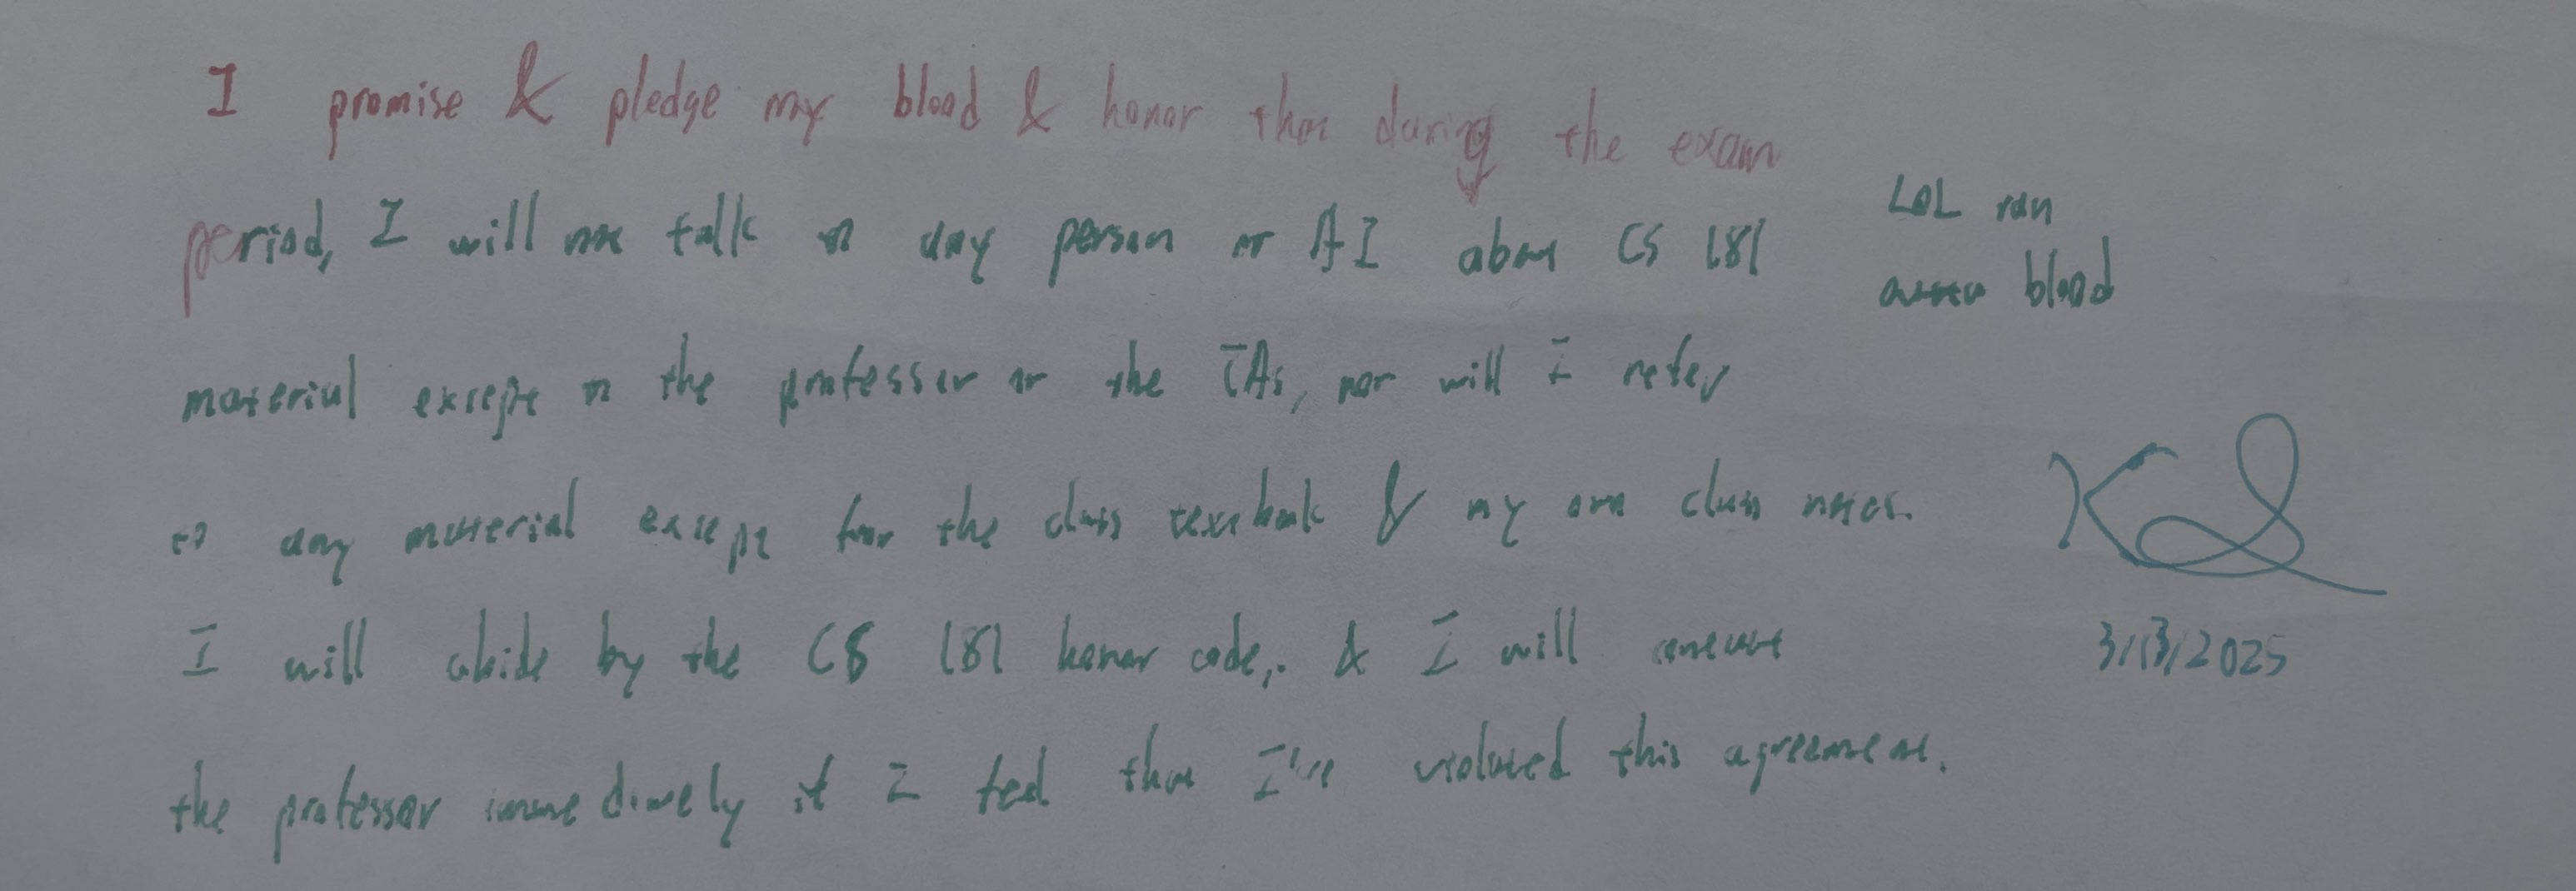
\includegraphics[width=15cm]{honor.jpg}
\end{center}

\pagebreak

\section{Singing Turing Machines}

\subsection{Ordinary Singer}\label{sec:ordsinger}

BWOC say there existed a recognizer $R$ for OrdinarySinger.

Then consider the following program:
\begin{algorithmic}[1]
    \Procedure{M}{$x$}
        \State $\alpha \gets \Braket{M}$
        \Comment{Get our own description by the Recursion Thm}
        \State Run $R(\alpha)$ for $|x|$ steps
        \If{$R$ is in an accepting state}
            \LComment{
                $R$ thinks we halt on all inputs, but we loop for all strings
                whose length is greater than the number of steps it takes for $R$ to halt.
            }
            \State Loop forever
        \Else
            \LComment{
                If $R$ rejects, we'll halt on all inputs with $ABC \subseteq \mathcal{N}^*$ on the song tape. \\
                If it loops (which counts as a rejection), the same thing will happen.
            }
            \State Write the string $ABC$ onto the song tape
            \State Accept
        \EndIf
    \EndProcedure
\end{algorithmic}
As indicated by the comments, no matter the behavior of $R$ on $M$,
it's behavior will always contradict the recognizer,
so the language is unrecognizable. $\square$

\pagebreak

\subsection{Infinite Singer}

A lot of this was copied straight from \ref{sec:ordsinger}; it is what it is.

BWOC say there existed a recognizer $R$ for InfiniteSinger.

Then consider the following program:
\begin{algorithmic}[1]
    \Procedure{M}{$x$}
        \State $\alpha \gets \Braket{M}$
        \State Run $R(\alpha)$ for $|x|$ steps
        \If{$R$ is in an accepting state}
            \LComment{
                $R$ thinks we loop on all inputs, but we halt on all strings
                whose length is greater than the number of steps it takes for $R$ to halt.
            }
            \State Accept
        \Else
            \LComment{
                If $R$ rejects, we'll write $A$s on the song tape until the end of time. \\
                If it loops (which counts as a rejection), the same thing will happen. \\
                Either way, $M$ will exhibit infinite singer behavior on all inputs when $R$ thinks it doesn't.
            }
            \For{$n \in \N$}
                \State Write $A$ on the song tape
                \State Move the song tape head to the right
            \EndFor    
        \EndIf
    \EndProcedure
\end{algorithmic}
As indicated by the comments, no matter the behavior of $R$ on $M$,
it's behavior will always contradict the recognizer,
so the language is unrecognizable. $\square$

\pagebreak

\section{Modify-Me Machines}

\subsection{Not Modify-Me Decidable}

% TODO: explain this better

Since everything given in the Modify-Me TM (MMTM) spec is finite, there is a countably
infinite number of Modify-Me TMS and we can bijectively map them to $\N$.

There's also a countably infinite number of finite-length binary strings,
so we can bijectively map those to $\N$ as well.
Then, with $\N$ as a middleman of sorts, we can construct a bijection
from the set of all MMTMs to the set of all input strings.

There's also a contably infinite number of finite-length binary strings, so consider
the infinite-site matrix $M$, where
\[M_{ij}=\begin{cases}
    1 & \text{The $i$th MMTM accepts the $j$th input string} \\
    0 & \text{otherwise}
\end{cases}\]
Notice that the $j$th input string in this case represents the encoding of the $j$th MMTM as well.

Now consider the language $H$, where the $i$th input string is in it if and only if $M_{ii}=0$.
In other words, using our bijective mappings, we can say
\[H=\{\braket{M} \mid \text{$M$ rejects itself}\}\]

$H$ is not equivalent to the language of any MMTM.
This is because for all $n \in \N$, if the $n$th MTM accepts the $n$th input string
$H$ should reject it, and if the machine rejects the string $H$ should accept it.

So here we've seen that the problem of whether an MMTM rejects itself is undecidable.

\pagebreak

\subsection{Co-HALT Decidability}

Here's an MMTM that solves Co-HALT:
\begin{algorithmic}[1]
    \Procedure{\texttt{CoHALT}}{$M$}
        \Procedure{N}{}
            \State Run $M(\epsilon)$
        \EndProcedure

        \item[]
        \State Write $\Braket{N}$ onto the machine tape
        \State GOTO $q_{\text{modify}}$
        \If{at $q_{\text{mod.done}}$}
            \State Reject
            \Comment{This means $M(\epsilon)$ halted and so $\Braket{M} \notin \text{Co-HALT}$}
        \ElsIf{at $q_{\text{mod.fail}}$}
            \State Accept
            \Comment{$M(\epsilon)$ runs infinitely so $\Braket{M} \in \text{Co-HALT}$}
        \EndIf
    \EndProcedure
\end{algorithmic}

\pagebreak

\subsection{EMPTY Decidability}

Here's an MMTM that solves EMPTY:
\begin{algorithmic}[1]
    \Procedure{\texttt{EMPTY}}{$M$}
        \Procedure{N}{}
            \State Run $M$ on all input strings with triangular scheduling
            \If{$\exists x \in \Sigma^*: M(x)$ accepts}
                \State \Return
            \Else
                \LComment{If no such $x$ exists, $N$ will loop until the heat death of the universe.}
            \EndIf
        \EndProcedure

        \item[]
        \State Write $\Braket{N}$ onto the machine tape
        \State GOTO $q_{\text{modify}}$
        \If{at $q_{\text{mod.done}}$}
            \State Reject
            \Comment{$N\text{ halted} \implies L(M) \ne \varnothing \implies \Braket{M} \notin \text{EMPTY}$}
        \ElsIf{at $q_{\text{mod.fail}}$}
            \State Accept
            \Comment{$N\text{ loops} \implies L(M)=\varnothing \implies \Braket{M} \in \text{EMPTY}$}
        \EndIf
    \EndProcedure
\end{algorithmic}

\pagebreak

\subsection{SINGLETON Decidability}\label{sec:singleton}

Let's assign each input string to a natural number.
In other words, we define a bijection $s(n): \N \to \Sigma^*$.
WIth that, we can write our MMTM like so:
\begin{algorithmic}[1]
    \Procedure{\texttt{SINGLETON}}{$M$}
        \LComment{\texttt{end} can be $\infty$! Indicate it with a special symbol or something.}
        \Procedure{N}{\texttt{start}, \texttt{end}}
            \State Run $M$ on all $s(n)$ s.t. $\texttt{start} < n < \texttt{end}$ with triangular scheduling
            \If{$\exists n: M(s(n))$ accepts}
                \State Write $n$ onto the work tape
                \State \Return
            \Else
                \LComment{
                    If no such $n$ exists, $N$ will loop forever or hit this else statement,
                    in which case we'll add a manual infinite loop to catch those cases.
                }
                \State Loop forever
            \EndIf
        \EndProcedure

        \item[]
        \State Write $\Braket{N}$ on the machine tape
        \State Make $\texttt{start}=0$ and $\texttt{end}=\infty$ and  on the work tape
        \State GOTO $q_{\text{modify}}$
        \If{at $q_{\text{mod.fail}}$}
            \State Reject
            \Comment{$N\text{ loops} \implies L(M)=\varnothing \implies \Braket{M} \notin \text{SINGLETON}$}
        \EndIf
     
        \item[]
        \State $x \gets$ content on work tape
        \Comment{$N$ returns some input that $M$ will accept.}

        \item[]
        \State Make $\texttt{start}=0$ and $\texttt{end}=x$ on work tape
        \State GOTO $q_{\text{modify}}$
        \If{at $q_{\text{mod.done}}$}
            \State Reject
            \Comment{$\exists y < x: M(x)\text{ accepts} \implies |L(M)| \ge 2$}
        \EndIf

        \item[]
        \State Make $\texttt{start}=x$ and $\texttt{end}=\infty$ on work tape
        \State GOTO $q_{\text{modify}}$
        \If{at $q_{\text{mod.done}}$}
            \State Reject
            \Comment{$\exists y > x: M(x)\text{ accepts} \implies |L(M)| \ge 2$}
        \EndIf

        \item[]
        \State Accept
    \EndProcedure
\end{algorithmic}

$N$ takes in a possibly infinite range of inputs (represented as natural numbers)
and tries to find an input in it which $M$ accepts.

If we find an input which $M$ accepts (lines 11-15), we rerun $N$
with the ranges to the left and to the right of $x$ to make sure
that the one we found is also the \textit{only} accepted one.

\pagebreak

\subsection{\texorpdfstring{$\text{LOOP}_{\text{ANY}}$}{LOOP\_ANY} Recognizability}

Oh, this one is actually easier than the last one:
\begin{algorithmic}[1]
    \Procedure{$\texttt{LOOP}_\texttt{ANY}$}{$M$}
        \Procedure{N}{$x$}
            \State Run $M(x)$
        \EndProcedure

        \item[]
        \For{all input strings $x$}
            \State Write $\Braket{N}$ onto the machine tape
            \State Write $x$ onto the work tape
            \State GOTO $q_{\text{modify}}$
            \If{at $q_{\text{mod.fail}}$}
                \State Accept
                \Comment{$N\text{ loops} \implies M(x)\text{ loops} \implies \Braket{M} \in \text{LOOP}_{\text{ANY}}$}
            \EndIf
        \EndFor
    \EndProcedure
\end{algorithmic}

If $M$ halts on all inputs, then this MMTM will loop forever.

\pagebreak

\subsection{FINITE Recognizability}

This MMTM uses a procedure that was already defined in \ref{sec:singleton}.
Redundancy be damned, I'm copy-pasting it here again:
\begin{algorithmic}[1]
    \Procedure{\texttt{FINITE}}{$M$}
        \Procedure{N}{\texttt{start}}
            \State Run $M$ on all $s(n)$ s.t. $n > \texttt{start}$ with triangular scheduling
            \If{$\exists n > \texttt{start}: M(s(n))$ accepts}
                \State Write $n$ onto the work tape
                \State \Return
            \Else
                \LComment{If no such $n$ exists, $N$ will loop until the heat death of the universe.}
            \EndIf
        \EndProcedure

        \item[]
        \State Write $\Braket{N}$ onto the machine tape
        \For{$n \in \{1, 2, 3, \cdots\}$}
            \State Make $\texttt{start}=n$ on work tape
            \State GOTO $q_{\text{modify}}$
            \Comment{Check if there's anything past \texttt{start} that's also accepted.}
            \If{at $q_{\text{mod.fail}}$}
                \LComment{$\exists N \in \N: M(s(i))$ doesn't accept for all $i > N$, so $|L(M)| < \infty$.}
                \State Accept
            \EndIf
        \EndFor
    \EndProcedure
\end{algorithmic}

\pagebreak

\section{Song Remixing}

I propose that if we can solve this, we can decide whether a TM halts.
To do this, we need to find some conversion method from a standard TM
to an instance of this problem.

\subsection{Tape Representation}\label{sec:encodings}

As long as we can encode $(Q \cup \{\text{no head}\}) \times \Gamma$,
which repsents the machine state and tape contents, we're golden.

\subsubsection{Encoding Head/State}\label{sec:tmstate}

We can use multiple characters to represent each state.

Let $n \in \N$ be so that $\binom{2n-1}{n-2} > |Q|$.
This allows us to construct an injective mapping from $Q$ to the set
\[\{s \in \{B, C\}^{2n-1} \mid \text{$s$ has exactly n Cs}\}\]
Now we can take each $q$ and transform it as follows:
\begin{itemize}[nolistsep]
    \item If $q$ is a halting state, force the first character to be $C$
          and map the remaining $n$ characters to something in $\{B, C\}^{2n-1}$ with exactly $n-1$ Cs.
    \item Otherwise, make it $B$ and map the tail to something in $\{B, C\}^{2n-1}$. with exactly $n$ Cs.
\end{itemize}

If the state we're encoding is "no head", then we'll just encode it with a string of $n$ As.

Define $f(q): (Q \cup \{\text{no head}\}) \to \{A, B, C\}^n$ as the injective function
that turns the state of the TM itself into a string of length $n$.

\subsubsection{Encoding \texorpdfstring{$\Gamma$}{Gamma}}

IDK what the blank symbol is- I'll just use $\varnothing$ as a placeholder.

Assume WLOG $\Gamma=\{0, 1, \varnothing\}$.
Then we can just tack on an $DEE$ for $0$, $EDE$ for $1$, or $EED$ for $\varnothing$
to the end of the string to represent the contents of the cell.

There's no real need for functions here- when I refer to something in $\Gamma$
from now on it'll be equivalent to the string I use to represent it.

\subsubsection{Preparation for Rules}

Since everything in $Q \cup \{\text{no head}\}$ is represented with exactly $2n$
characters and the cell content is just two more characters,
all tape cells are of uniform size.

For reasons, we'll append an F to each tape cell as well.

Also, for convenience let $l$ represent the length of the string
we use to represent each cell.

\pagebreak

\subsection{Initial Condition}

We'll try to simulate $M(\epsilon)$ for any TM $M$.
To do this, we'll let $s_0$ be just $l$ characters:
\[\text{string representing $q_0$} \mid EEDF\]
(The pipe in the middle represents concatenation).

This string represents a single tape cell containing $\varnothing$
with the head pointed at it and the machine at $q_0$.

\subsection{Song to Append}

We'll define $s_A$ as follows:
\[s_A=\underbrace{AA \cdots A}_{\text{$n$ As}}EEDF\]
which represents a cell with blank contents and the head not pointed at it.

At the start (or during execution, it doesn't really matter)
we can give ourselves however much "memory" we want.
If the head tries to move right when there's no more tape cells,
we append the thing from $s_A$ and continue.

\subsection{Rules}

For all $a, b \in Q$ and $c, d, e \in \Gamma$ s.t. $\delta(a, c)=(b, d, R)$, we should add the tuple
\[f(a) \mid c \mid F \mid f(\text{no head}) \mid e \mid F \to_R f(\text{no head}) \mid d \mid F \mid f(b) \mid e \mid F\]
where $f$ is the function defined in \ref{sec:tmstate}.

We can define something similar where all the variables are the same except this time it's $\delta(a, c)=(b, d, L)$,
where we just swap the order of the two cells:
\[f(\text{no head}) \mid e \mid F \mid f(a) \mid c \mid F \to_R f(b) \mid e \mid F \mid f(\text{no head}) \mid d \mid F\]

\pagebreak

\subsection{Rule Validity}

\subsubsection{Valid Permutations}

I'll only argue the case where we move right, because if we move left it's the same thing.

Let's take a look at what we have on each side of the rule:
\begin{multicols}{2}
    \textbf{LHS}
    \begin{itemize}[nolistsep]
        \item $f(a)$
        \item $c$
        \item $f(\text{no head})$
        \item $e$
        \item Two Fs
    \end{itemize}
    \columnbreak
    \textbf{RHS}
    \begin{itemize}[nolistsep]
        \item $f(\text{no head})$
        \item $d$
        \item $f(b)$
        \item $e$
        \item Two Fs
    \end{itemize}
\end{multicols}
Everything matches up except $f(a)$, $f(b)$, $c$, and $d$.

However, notice that due to how we encoded things in \ref{sec:encodings},
every output of $f$ (besides $f(\text{no head})$) has $n$ Bs and $n$ Cs,
and everything in $\Gamma$ is mapped to two Es and one D.
This means that $f(a)$ and $f(b)$ are permutations of one another,
and the same can be said for $c$ and $d$.

With that, we've proven the validity of all the remixing rules we've defined.

\subsubsection{Valid Simultation}

Also, each rule can only be used on two adjacent cells where the head is in one of them.
This is because of the F we added on at the suffix of each cell.

Any rule would have to end exactly with an F, and since all cells are of length $l$,
any rule will have to "hook onto" the end of a cell.

Notice that we can remix the song to something that starts with a C
if and only if the machine corresopnding to the remixing problem halts.
Since we assumed TMs halt at the leftmost point of the tape
and a state starts with a C iff it's a halting state,
if we've remixed the song the start with a C it means the TM's halted.

\pagebreak

\subsection{Finally, Undecidable}

For the final time, BWOC say there existed a decider $D$ for SongRemixing.

Then consider the following TM:
\begin{algorithmic}[1]
    \Procedure{M}{x}
        \State $\alpha \gets \Braket{M}$
        \State Convert $\alpha$ to an instance $\beta$ of SongRemixing by the rules we just made
        \If{$D(\beta)$ accepts}
            \State Loop forever
            \Comment{$D$ thinks we'll halt on $\epsilon$, but we'll actually loop}
        \ElsIf{$D(\beta)$ rejects}
            \State Halt
            \Comment{$D$ thinks we'll loop forever on $\epsilon$, but we'll actually halt}
        \EndIf
    \EndProcedure
\end{algorithmic}
As the comments show, $D$ must get the converted version of $\Braket{M}$ wrong,
so no such decider can exist. $\square$

\pagebreak

\section{EC Drawing}

I thought this drawing was good enough to warrant its own page.
Y'all are lookin' at the next Mona Lisa right here:
\begin{center}
    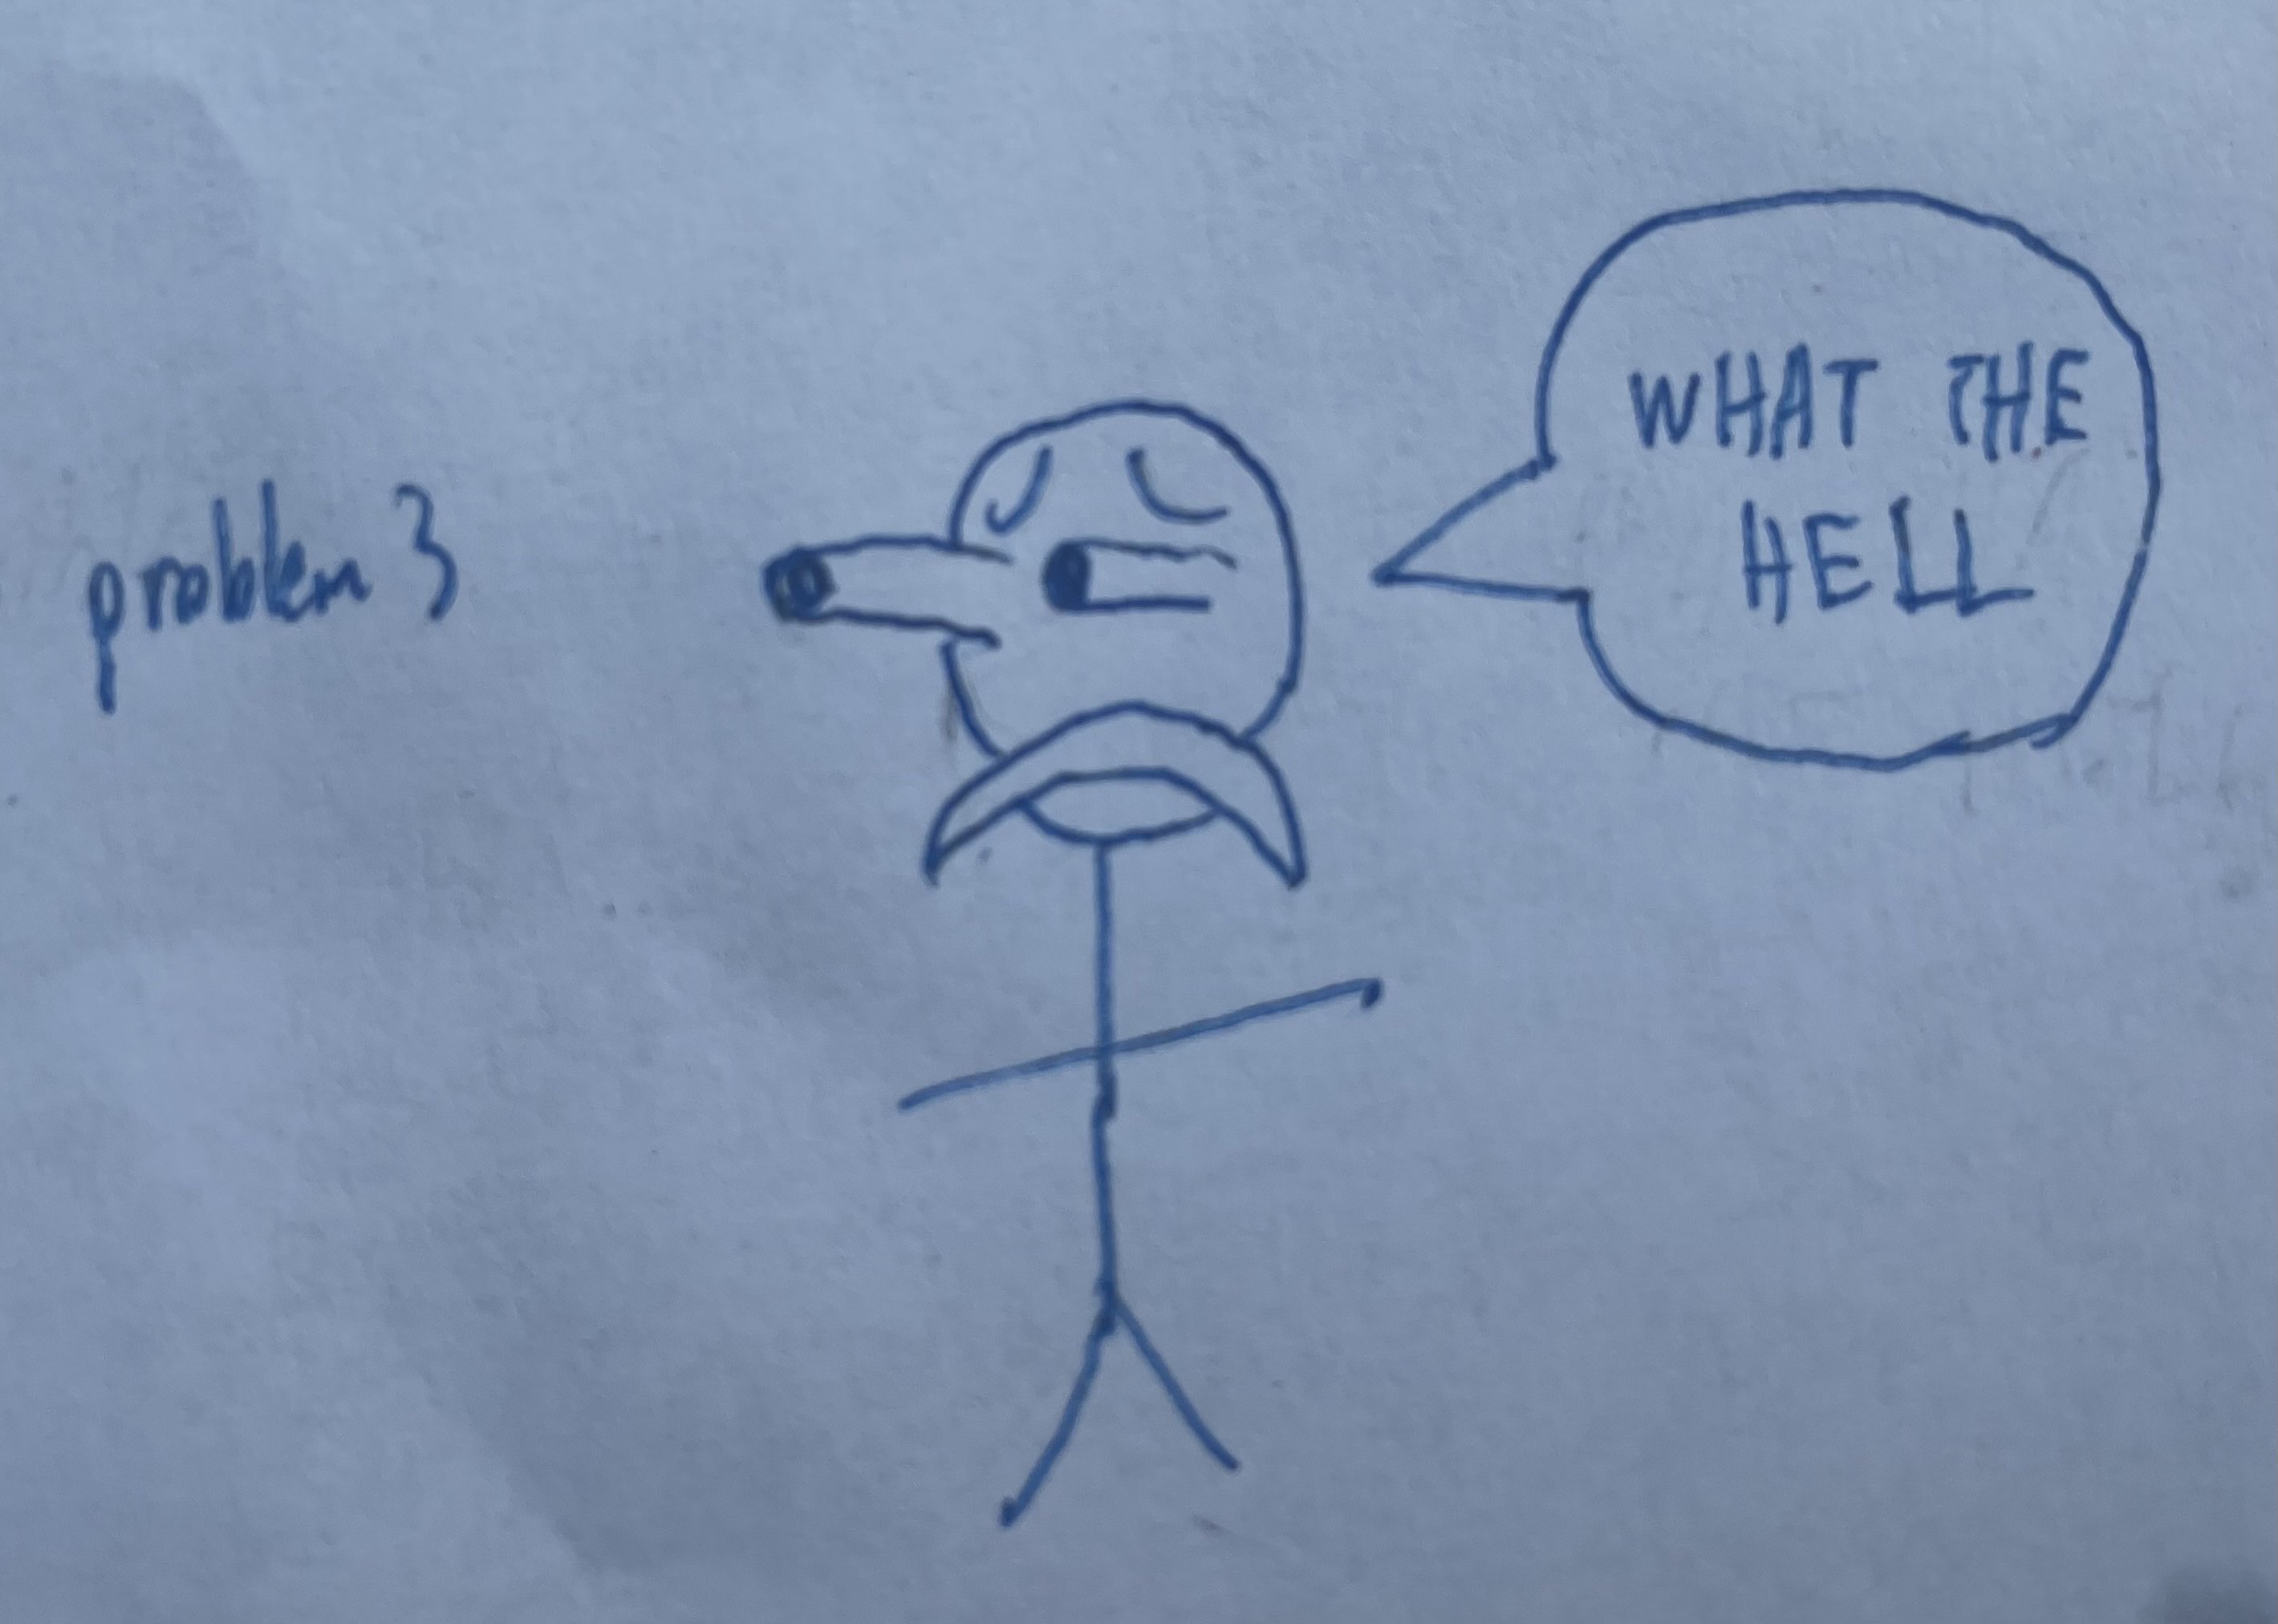
\includegraphics[width=15cm]{ec_drawing}
\end{center}

\end{document}
